\documentclass[12pt]{article}

\usepackage{amsmath, amsthm, amssymb,multirow}
\usepackage{algorithm}
\usepackage[noend]{algpseudocode}
\usepackage{amssymb,amsmath,amsthm,graphicx, amsfonts,latexsym,mathtext, array, enumerate, verbatim, hyperref, listings,color,geometry, caption, subcaption, dsfont}

\newtheorem{rem}{Remark}
\newcommand{\M}{\mathbf}
\newcommand{\B}{\boldsymbol}
\newcommand{\1}{\mathds{1}}


\begin{document}

\title{Homework 1}
 
\author{Ying Daisy Zhuo}
%
\maketitle

\section{Problem One}

I implemented the problem in JuMP. The formulations are as follows:
Original problem ($L_0$):
\begin{equation}
\begin{aligned}
\max ~~&\sum_{i=1}^n z_i &\\
\textrm{s.t.} ~~& \M A \M x = \M b		&\\
			 & |x_i| \leq M(1-z_i)& \forall i=1, 2, \ldots, n\\
			 & z_i \in \{0, 1\}		& \forall i=1, 2, \ldots, n\\
\end{aligned}
\end{equation}

$L_1$ relaxation problem:
\begin{equation}
\begin{aligned}
\min ~~&\sum_{i=1}^n x^+_i + x^-_i &\\
\textrm{s.t.} ~~& \M A (\M x^+ - \M x^-) = \M b		&\\
			 & x^+_i \geq 0	& \forall i=1, 2, \ldots, n\\
			 & x^-_i \geq 0 	& \forall i=1, 2, \ldots, n\\
\end{aligned}
\end{equation}


For fixed $n = 100$, we solve the problem for various $m=1, 10, \ldots, 100$ and $k = 1, 5, \ldots, m$. If the $L_1$ relaxation solves the problem and gets the same sparse solution as the solution to the true $L_0$ problem, then we indicate it as ``recovered". Figure \ref{fig:prob1} depicts whether the problem is recovered based on the ratio between $m$ and $n$ on the x-axis, and the ratio between $k$ and $m$ on the y-axis.

\begin{figure}
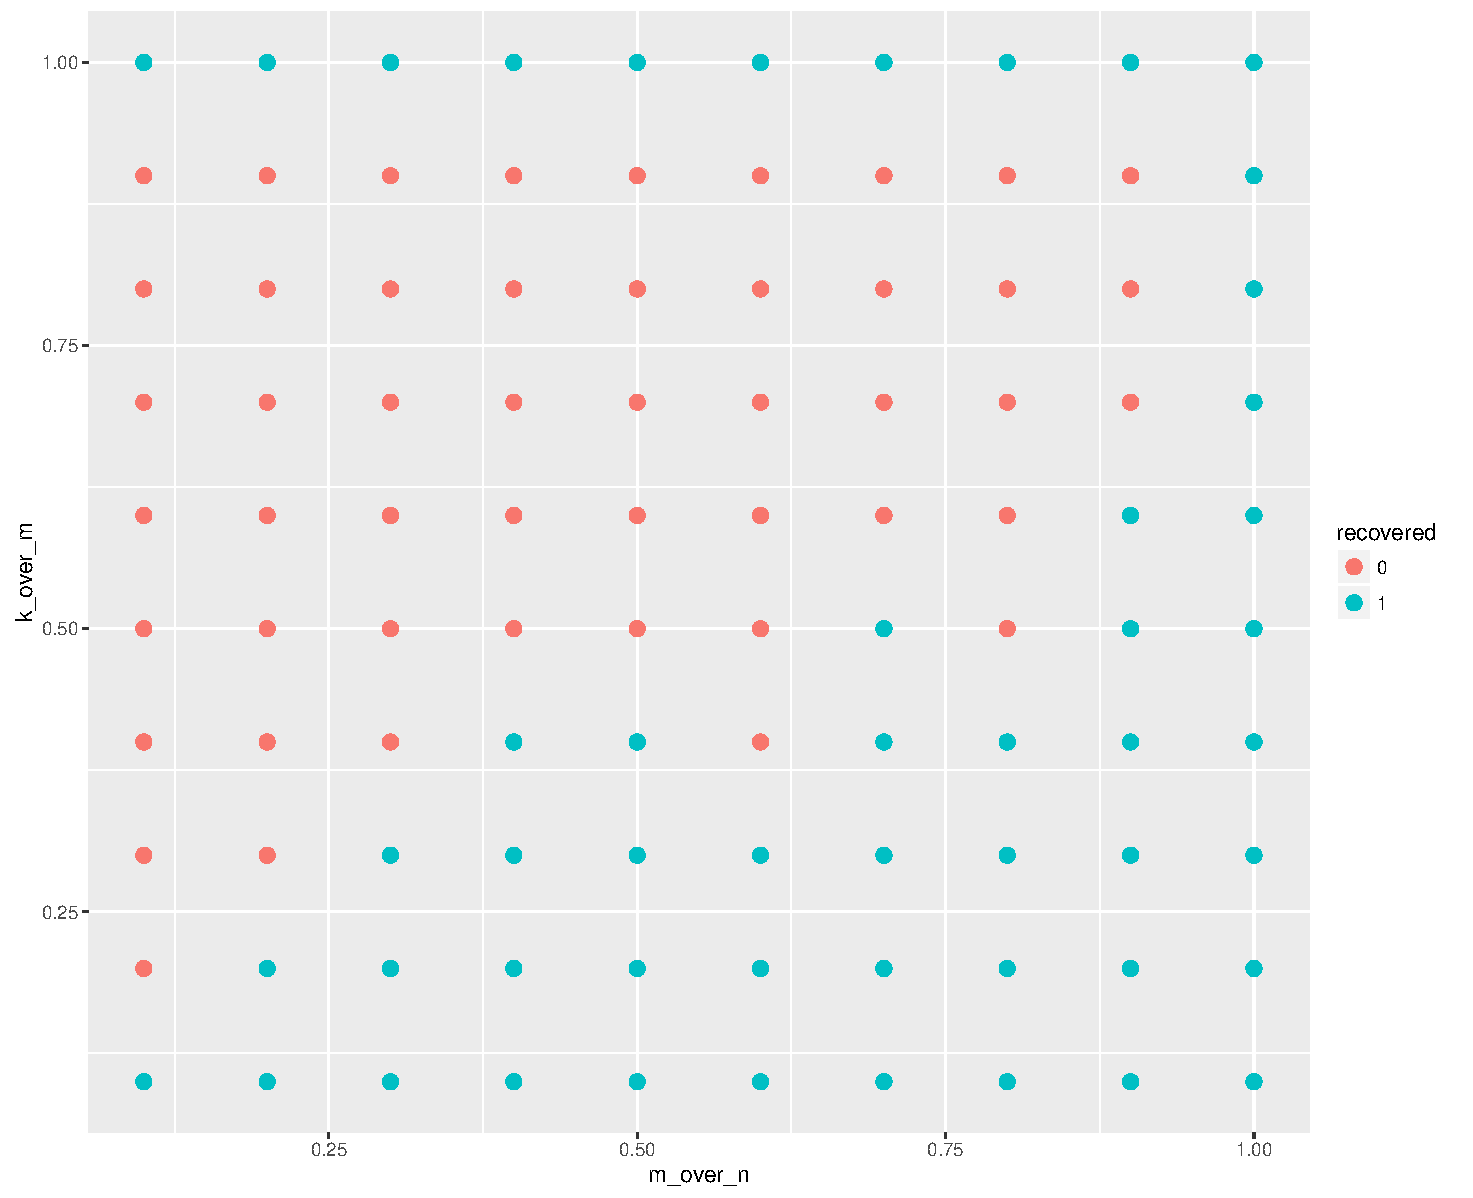
\includegraphics[scale=0.6]{hw1_output.pdf}
\caption{Plot of whether the sparse solution is recovered in the $L_1$ relaxation problem based on $m/n$ and $k/m$. }\label{fig:prob1}
\end{figure}

Observe that along the diagonal line, it separates the region into two areas. In the one to the lower right (with high $m/n$ and low $k/m$), $L_1$ can recover the true solution; in the one to the upper left (with low $m/n$ and high $k/m$), $L_1$ is unable to recover the true solution.


\newpage
\section{Problem Two}
In this problem, we are asked to formulate regression problems with some additional properties using MIO. In particular, some desirable properties include:
\begin{enumerate}
\item Pairwise multi-collinearity
\item Group sparsity
\item Sparsity
\item Robustness
\item Non-linear transformation
\item Statistical significance
\end{enumerate}

To do so, we need some pre-processing. First, we expand the dataset to include non-linear transformations. For this example, we include $x^2$ and $\log(x)$ for each of the data dimensions.  In addition, we compute the correlation matrix and obtain pairs $\{i,j\}$ of covariates that have correlation greater than a threshold, say $0.8$, and save the set of pairs $\mathcal{HC}$. 

We can now implement the first five items as the following problem:
\begin{equation}
\begin{aligned}
\min ~~&\sum_{i=1}^n \frac{1}{2}\|\M y-\M X \B\beta\| + \Gamma \|\B\beta \|_1 &\\
\textrm{s.t.} ~~& -M z_d \leq \B\beta_d \leq M z_d 	& \forall d=1, 2, \ldots, D\\
			 & \sum_{d=1}^D z_d \leq k &\\
			 & z_i + z_j \leq 1 &\forall \{i, j\} \in \mathcal{HC} \\
			 & \sum_{i\in \mathcal{T}_m} z_i\leq 1 &\forall m \\
			 & z_d \in \{0,1\}  	& \forall d=1, 2, \ldots, D\\
\end{aligned}\label{eq:prob2}
\end{equation}

The implementation of statistical significance is done in a iterative fashion. At we solve the initial Problem \ref{eq:prob2}, we run a simple linear model with all the variables selected and see if all variables are statistically significant. If so, do not add any constraint and terminate. Otherwise, add the following constraint:
$\sum z_i \leq current\_count - 1$ and solve the problem. Iterate until termination.

The parameters $\Gamma$ and $k$ can be tuned using cross validation. Using the \textit{lpga2009} dataset, we obtain an optimal solution with $\beta_11 = -11.395$ and the rest being zero. This give an out-of-sample $R^2$ of $0.80$.


\section{Problem Three}
Using the same technique from class, we find the following majorization of the first term:

\begin{equation}
g(\B\beta) \leq Q(\B\beta) = g(\B\beta_0) + \nabla g(\B\beta_0)^T (\B\beta - \B\beta_0) + \frac{L}{2} \| \B\beta - \B\beta_0\|^2,~~~\forall L \geq l,
\end{equation}

where $l$ is the Lipschitz constant on the first order derivative of $g$. We can solve the following problem:

\begin{equation}
\begin{aligned}
\min ~~&\sum_{i=1}^n \frac{L}{2}\|\B\beta - \M u\|^2  + \Gamma \| \B\beta\|_1 -\frac{1}{2L} \|\nabla g(\B\beta_0) \|^2&\\
\textrm{s.t.} ~~& \|\B\beta\| \leq k,
\end{aligned}\label{eq:prob2}
\end{equation}

where $u_i = \B\beta_0 - \frac{1}{L}\nabla g(\B\beta_0)$. Notice that the last term in the objective is a constant, and the rest of the objective term is separable. Therefore, for each $i$,
\begin{equation}
Q_i = \min ~~ \frac{L}{2} (\beta_i - u_i)^2+ \Gamma | \beta_i |^2
\end{equation}

To find the optimal solution to the above problem, we look at the following scenarios:
\begin{enumerate}
\item When $u_i \geq \Gamma/L$, optimality is achieved at $\beta_i = \Gamma/L - u_i$.
\item When $u_i \leq - \Gamma/L$, optimality is achieved at $\beta_i = \Gamma/L + u_i$.  
\item When $|u_i| \leq \Gamma/L$, $beta_i = 0$ achieves optimality.
\end{enumerate} 

We are now able to compute the objective $Q_i$ for each $i$. We then sort the $Q_i$'s and pick the k lowest values.





\end{document}
